\SourceLeaf{117}
alle aus dem Princip, dass die Producte aus den von einander abgekehrten (bloss
gemeinschaftliche Spitze habenden, oder noch concinner, keine gemeinschaftliche Seite
habenden) Dreiecken, in welche ein Viereck durch die Diagonalen zerlegt wird, gleich sind.

Die allgemeine barycentrische Gleichung zwischen vier Punkten, z.\,B. $(A)$, $(B)$, $(C)$,
$(D)$ ist:
\[
\TriLetter{A}\,(A)+\TriLetter{B}\,(B)+\TriLetter{C}\,(C)+\TriLetter{D}\,(D)=0,
\]
wo $\TriLetter{A}$ das Dreieck $BCD$, $\TriLetter{B}$ das Dreieck $CDA$
u.\,s.\,w. (mit Rücksicht auf [das] Zeichen) vorstellt. In unserm Fall wird, wenn man zu
obigen Bezeichnungen noch setzt:
\[
\boldsymbol{A}^{*}=\alpha+\gamma+\delta+a+\lambda, \quad \text{u.\,s.\,w.}
\]
\[
\boldsymbol{A}^{*}=\omega-\mathfrak{B}-\mathfrak{E}, \quad \text{u.\,s.\,w.},
\]
der Typus der Gleichung zwischen vier Punkten:
\[
\mathfrak{C}(A)+\boldsymbol{D}^{*}(C)=\boldsymbol{A}^{*}(B)+\mathfrak{B}(D),
\]
wo $(A)$ den betreffenden Eckpunkt des äussern Pentagons ausdrückt, oder:
\[
\begin{gathered}\mathfrak{C}(A)+(\omega-\mathfrak{E}-\mathfrak{C})(C)\\=(\omega-\mathfrak{B}-\mathfrak{E})(B)+\mathfrak{B}(D)\\=(\omega-\mathfrak{E})(e),\end{gathered}
\]
wo $(e)$ den betreffenden Punkt des inneren Pentagons ausdrückt.

\begin{center}\rule{3cm}{.4pt}\end{center}

\begin{center}\resizebox{7cm}{!}{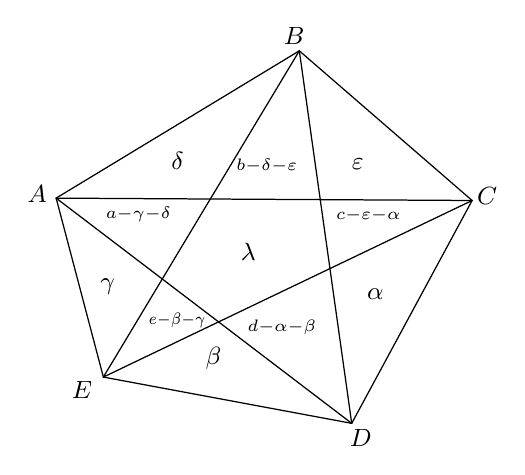
\begin{tikzpicture}[x=.006cm,y=-.006cm,line width=.45pt,line cap=round,line join=round,every node/.style={inner sep=0pt,font=\small}]
\coordinate (A) at (158,408);
\coordinate (B) at (673,96);
\coordinate (C) at (1039,413);
\coordinate (D) at (784,885);
\coordinate (E) at (258,787);
\draw (A) -- (B);
\draw (B) -- (C);
\draw (C) -- (D);
\draw (D) -- (E);
\draw (E) -- (A);
\draw (A) -- (C);
\draw (A) -- (D);
\draw (B) -- (E);
\draw (B) -- (D);
\draw (C) -- (E);
\node at (118,400) {$A$};
\node at (662,65) {$B$};
\node at (1071,403) {$C$};
\node at (803,916) {$D$};
\node at (213,814) {$E$};
\node at (415,330) {$\delta$};
\node at (604,339) {$\scriptstyle b-\delta-\varepsilon$};
\node at (797,337) {$\varepsilon$};
\node at (332,443) {$\scriptstyle a-\gamma-\delta$};
\node at (819,445) {$\scriptstyle c-\varepsilon-\alpha$};
\node at (565,522) {$\lambda$};
\node at (267,596) {$\gamma$};
\node at (414,666) {\scalebox{.86}[1]{$\scriptstyle e-\beta-\gamma$}};
\node at (491,747) {$\beta$};
\node at (636,681) {$\scriptstyle d-\alpha-\beta$};
\node at (834,612) {$\alpha$};
\end{tikzpicture}
}\end{center}

\[
\boldsymbol{A}c\varepsilon+\boldsymbol{C}c(b-\varepsilon)=\boldsymbol{B}b(c-\varepsilon)+\boldsymbol{D}b\varepsilon,
\]
\[
\boldsymbol{B}d\alpha+\boldsymbol{D}d(c-\alpha)=\boldsymbol{C}c(d-\alpha)+\boldsymbol{E}c\alpha,
\]
\[
\boldsymbol{C}e\beta+\boldsymbol{E}e(d-\beta)=\boldsymbol{D}d(e-\beta)+\boldsymbol{A}d\beta,
\]
\[
\boldsymbol{D}a\gamma+\boldsymbol{A}a(e-\gamma)=\boldsymbol{E}e(a-\gamma)+\boldsymbol{B}e\gamma,
\]
\[
\boldsymbol{E}b\delta+\boldsymbol{B}b(a-\delta)=\boldsymbol{A}a(b-\delta)+\boldsymbol{C}a\delta,
\]
